\begin{figure}[H]
    \centering
    \caption{Quadrant Size and Police Cases}
    \label{fig:quadrantsize}
    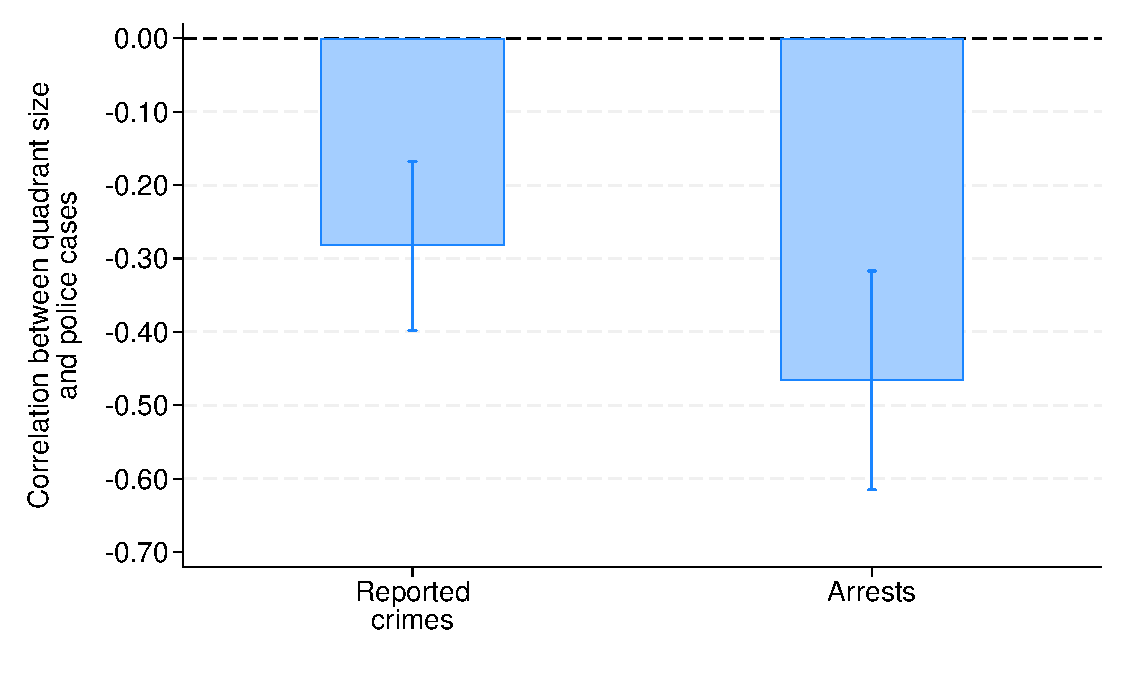
\includegraphics[width=0.75\textwidth]{../manuscript/Graphs/quadrantsize_crime.pdf}
    \\[12pt]
    \begin{minipage}{0.99\textwidth}
    Notes: Each bar reports the coefficient on quadrant size from a separate regression of the number of police cases in a quadrant and year, with municipality and year fixed effects. Both variables are in logarithms, so each bar is an elasticity: the percentage change in police cases associated with a one percent larger quadrant. The bars display 95\% confidence intervals, with standard errors clustered at the municipality level.
    \end{minipage}
\end{figure}
